\documentclass[tikz]{standalone}
\usepackage{tikz}
\usepackage{xcolor} % For custom colors

\begin{document}

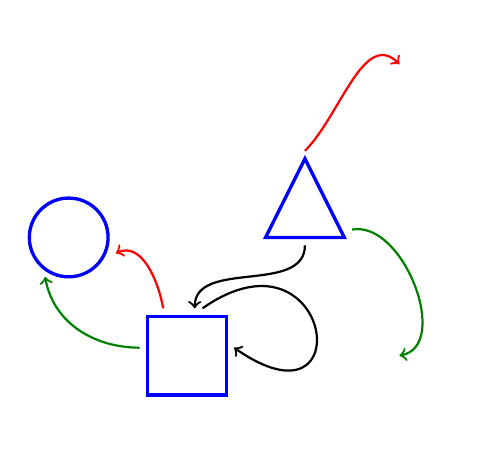
\begin{tikzpicture}
    % Define a less vibrant green
    \definecolor{mygreen}{rgb}{0.0, 0.5, 0.0} % Darker, muted green

    % Draw a blue square
    \draw[draw=blue, very thick] (2,0) rectangle (1,1);

    % Draw a blue triangle
    \draw[draw=blue, very thick] (2.5,2) -- (3.5,2) -- (3,3) -- cycle;

    % Draw a blue circle
    \draw[draw=blue, very thick] (0,2) circle (0.5);

    % Arrows from the square to the circle (slightly offset)
    \draw[->, thick, red] (1.2,1.1) to[out=100, in=25] (.6,1.8); 
    \draw[->, thick, mygreen] (.9,0.6) to[out=180, in=-80] (-0.3,1.5);

    % Circular arrow from the square to itself (offset slightly)
    \draw[->, thick, black] (1.7,1.1) to[out=35, in=-35, looseness=8] (2.1,.6);

    % Arrow from the triangle to the square (slightly offset)
    \draw[->, thick, black] (3,1.9) to[out=-90, in=90] (1.6,1.1);

    % Arrows from the triangle to nowhere (slightly offset)
    \draw[->, thick, red] (3,3.1) to[out=45, in=135] (4.2,4.2);
    \draw[->, thick, mygreen] (3.6,2.1) to[out=10, in=10] (4.2,.5);

\end{tikzpicture}

\end{document}
